%\documentclass[a4paper]{article}
%\usepackage[margin=0pt]{geometry}
%\usepackage{nopageno}
\documentclass[varwidth, border=4pt]{standalone}
\usepackage{tikz}
\usepackage{amsmath}
\usepackage{xspace}
\usepackage{bm}
\usetikzlibrary{positioning, arrows.meta, bending, fit, calc, decorations.pathmorphing}
\begin{document}
%\thispagestyle{empty}

\begin{standalone}
\begin{figure}
\center
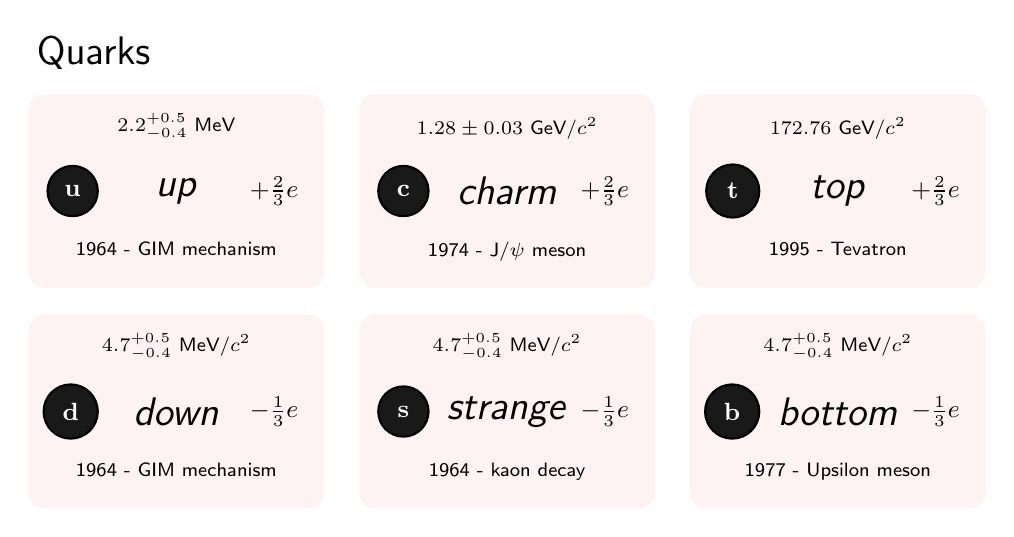
\begin{tikzpicture}[scale=1.4,font=\sffamily\small,rectangle/.style={fill=pink!20, rounded corners=.2cm},box/.style={rounded corners=.2cm}]


  \node[box] (quarks) at (-0.75,1.25) {\Large Quarks};

  % Define quarks
  \node[rectangle,text centered,text width = 0.29\textwidth, minimum height=7em,] (up) at (0,0) {\Large \textit{up}};
  \node[rectangle,text centered,text width = 0.29\textwidth, minimum height=7em,] (charm) at (3,0) {\Large \textit{charm}};
  \node[rectangle,text centered,text width = 0.29\textwidth, minimum height=7em,] (top) at (6,0) {\Large \textit{top}};
  \node[rectangle,text centered,text width = 0.29\textwidth, minimum height=7em,] (down) at (0,-2) {\Large \textit{down}};
  \node[rectangle,text centered,text width = 0.29\textwidth, minimum height=7em,] (strange) at (3,-2) {\Large \textit{strange}};
  \node[rectangle,text centered,text width = 0.29\textwidth, minimum height=7em,] (bottom) at (6,-2) {\Large \textit{bottom}};

  % Mass
  \node[above=1.5em of up.center] {\scriptsize $2.2^{+0.5}_{-0.4}$ MeV};
  \node[above=1.5em of charm.center] {\scriptsize $1.28 \pm 0.03$ GeV/$c^2$};
  \node[above=1.5em of top.center] {\scriptsize $172.76$ GeV/$c^2$};
  \node[above=1.5em of down.center] {\scriptsize $4.7^{+0.5}_{-0.4}$ MeV/$c^2$};
  \node[above=1.5em of strange.center] {\scriptsize $4.7^{+0.5}_{-0.4}$ MeV/$c^2$};
  \node[above=1.5em of bottom.center] {\scriptsize $4.7^{+0.5}_{-0.4}$ MeV/$c^2$};

  % Electric charge
  \node[right=2.3em of up.center] {$+\frac{2}{3} e$};
  \node[right=2.3em of charm.center] {$+\frac{2}{3} e$};
  \node[right=2.3em of top.center] {$+\frac{2}{3} e$};
  \node[right=2.3em of down.center] {$-\frac{1}{3} e$};
  \node[right=2.3em of strange.center] {$-\frac{1}{3} e$};
  \node[right=2.3em of bottom.center] {$-\frac{1}{3} e$};

  % Symbol
  \node[draw,circle,text width=0.8em,align=center,thick,fill=black!90,text=white,left=2.8em of up.center] {$\mathbf{u}$};
  \node[draw,circle,text width=0.8em,align=center,thick,fill=black!90,text=white,left=2.8em of charm.center] {$\mathbf{c}$};
  \node[draw,circle,text width=0.8em,align=center,thick,fill=black!90,text=white,left=2.8em of top.center] {$\mathbf{t}$};
  \node[draw,circle,text width=0.8em,align=center,thick,fill=black!90,text=white,left=2.8em of down.center] {$\mathbf{d}$};
  \node[draw,circle,text width=0.8em,align=center,thick,fill=black!90,text=white,left=2.8em of strange.center] {$\mathbf{s}$};
  \node[draw,circle,text width=0.8em,align=center,thick,fill=black!90,text=white,left=2.8em of bottom.center] {$\mathbf{b}$};

  % Discovery
  \node[below=1.5em of up.center] {\scriptsize 1964 - GIM mechanism};
  \node[below=1.5em of charm.center] {\scriptsize 1974 - J/$\psi$ meson};
  \node[below=1.5em of top.center] {\scriptsize 1995 - Tevatron};
  \node[below=1.5em of down.center] {\scriptsize 1964 - GIM mechanism};
  \node[below=1.5em of strange.center] {\scriptsize 1964 - kaon decay};
  \node[below=1.5em of bottom.center] {\scriptsize 1977 - Upsilon meson};
\end{tikzpicture}
%%%%%%%%%%%%%%%%%%%%
\vspace{0.2em}\\
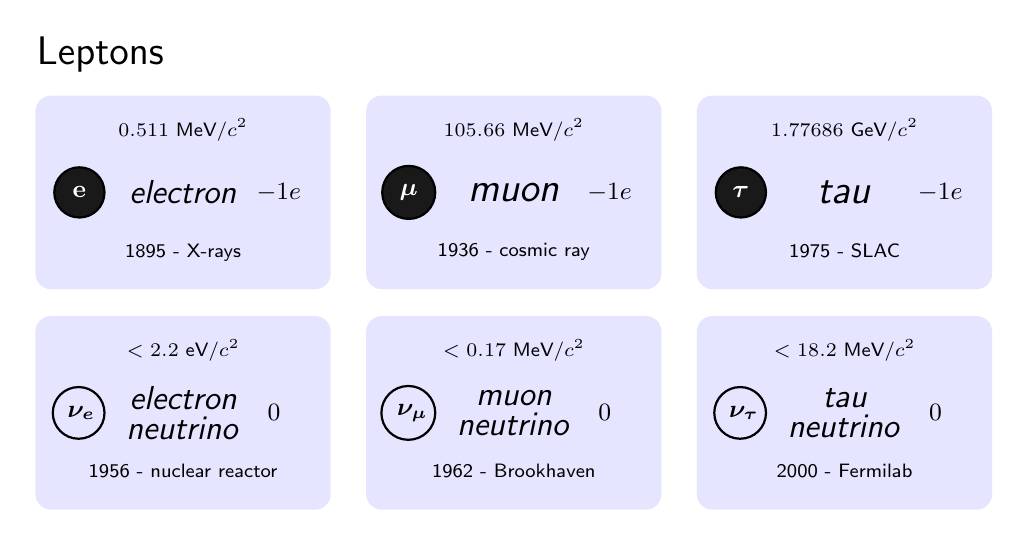
\begin{tikzpicture}[scale=1.4,font=\sffamily\small,rectangle/.style={fill=blue!10, rounded corners=.2cm},box/.style={rounded corners=.2cm}]

\node[box] (leptons) at (-0.75,1.25) {\Large Leptons};

% Define leptons
\node[rectangle,text centered,text width = 0.29\textwidth, minimum height=7em,] (electron) at (0,0) {\large \textit{electron}};
\node[rectangle,text centered,text width = 0.29\textwidth, minimum height=7em,] (muon) at (3,0) {\Large \textit{muon}};
\node[rectangle,text centered,text width = 0.29\textwidth, minimum height=7em,] (tau) at (6,0) {\Large \textit{tau}};
\node[rectangle,text centered,text width = 0.29\textwidth, minimum height=7em,] (electron_neutrino) at (0,-2) {\large \textit{electron\\neutrino}};
\node[rectangle,text centered,text width = 0.29\textwidth, minimum height=7em,] (muon_neutrino) at (3,-2) {\large \textit{muon\\neutrino}};
\node[rectangle,text centered,text width = 0.29\textwidth, minimum height=7em,] (tau_neutrino) at (6,-2) {\large \textit{tau\\neutrino}};

% Mass
\node[above=1.5em of electron.center] {\scriptsize $0.511$ MeV/$c^2$};
\node[above=1.5em of muon.center] {\scriptsize $105.66$ MeV/$c^2$};
\node[above=1.5em of tau.center] {\scriptsize $1.77686$ GeV/$c^2$};
\node[above=1.5em of electron_neutrino.center] {\scriptsize $< 2.2$ eV/$c^2$};
\node[above=1.5em of muon_neutrino.center] {\scriptsize $< 0.17$ MeV/$c^2$};
\node[above=1.5em of tau_neutrino.center] {\scriptsize $< 18.2$ MeV/$c^2$};

% Electric charge
\node[right=2.3em of electron.center] {$-1 e$};
\node[right=2.3em of muon.center] {$-1 e$};
\node[right=2.3em of tau.center] {$-1 e$};
\node[right=2.7em of electron_neutrino.center] {$0$};
\node[right=2.7em of muon_neutrino.center] {$0$};
\node[right=2.7em of tau_neutrino.center] {$0$};

% Symbol
\node[draw,circle,text width=0.8em,align=center,thick,fill=black!90,text=white,left=2.8em of electron.center]{$\mathbf{e}$};
\node[draw,circle,text width=0.8em,align=center,thick,fill=black!90,text=white,left=2.8em of muon.center]{$\bm{\mu}$};
\node[draw,circle,text width=0.8em,align=center,thick,fill=black!90,text=white,left=2.8em of tau.center]{$\bm{\tau}$};
\node[draw,circle,text width=0.8em,align=center,text width=0.8em,thick,left=2.8em of electron_neutrino.center]{$\bm{\nu_e}$};
\node[draw,circle,text width=0.8em,align=center,thick,left=2.8em of muon_neutrino.center]{$\bm{\nu_\mu}$};
\node[draw,circle,text width=0.8em,align=center,thick,left=2.8em of tau_neutrino.center]{$\bm{\nu_\tau}$};

% Discovery
\node[below=1.5em of electron.center] {\scriptsize 1895 - X-rays};
\node[below=1.5em of muon.center] {\scriptsize 1936 - cosmic ray};
\node[below=1.5em of tau.center] {\scriptsize 1975 - SLAC};
\node[below=1.5em of electron_neutrino.center] {\scriptsize 1956 - nuclear reactor};
\node[below=1.5em of muon_neutrino.center] {\scriptsize 1962 - Brookhaven};
\node[below=1.5em of tau_neutrino.center] {\scriptsize 2000 - Fermilab};
\end{tikzpicture}
%%%%%%%%%%%%%
\vspace{0.2em}\\
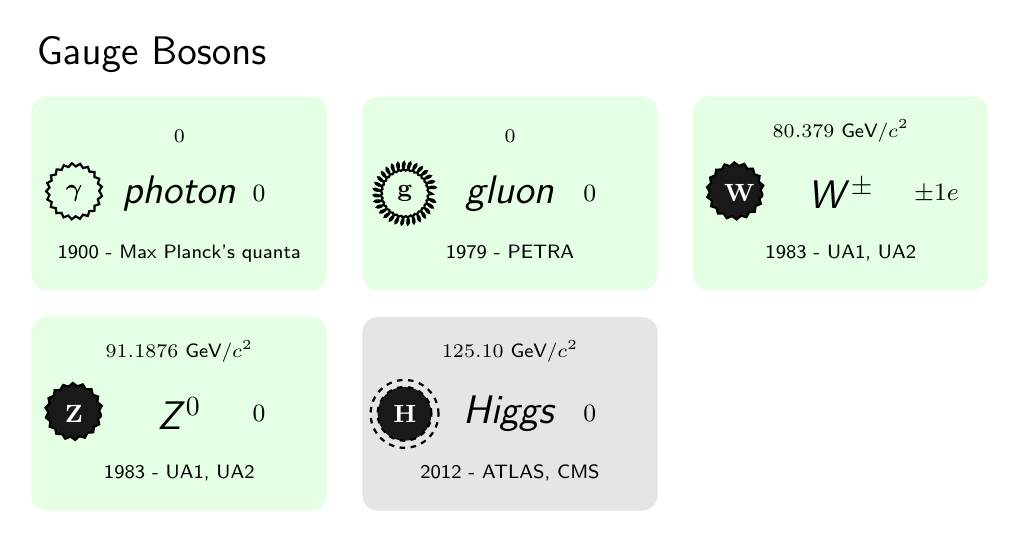
\begin{tikzpicture}[scale=1.4,font=\sffamily\small,rectangle/.style={fill=green!10, rounded corners=.2cm},box/.style={rounded corners=.2cm}]



% Define bosons
\node[rectangle,text centered,text width = 0.29\textwidth, minimum height=7em,] (photon) at (0,0) {\Large \textit{photon}};
\node[rectangle,text centered,text width = 0.29\textwidth, minimum height=7em,] (gluon) at (3,0) {\Large \textit{gluon}};
\node[rectangle,text centered,text width = 0.29\textwidth, minimum height=7em,] (W) at (6,0) {\Large \textit{W}$^{\pm}$};
\node[rectangle,text centered,text width = 0.29\textwidth, minimum height=7em,] (Z) at (0,-2) {\Large \textit{Z}$^{0}$};
\node[rectangle,fill=black!10,text centered,text width = 0.29\textwidth, minimum height=7em,] (Higgs) at (3,-2) {\Large \textit{Higgs}};
%\node[rectangle,text centered,text width = 0.29\textwidth, minimum height=7em,] (graviton) at (6,-2) {\Large \textit{Higgs}};

\node[box, above=0.5em of photon, xshift=-1em] (bosons){\Large Gauge Bosons};

% Mass
\node[above=1.5em of photon.center] {\scriptsize $0$};
\node[above=1.5em of gluon.center] {\scriptsize $0$};
\node[above=1.5em of W.center] {\scriptsize $80.379$ GeV/$c^2$};
\node[above=1.5em of Z.center] {\scriptsize $91.1876$ GeV/$c^2$};
\node[above=1.5em of Higgs.center] {\scriptsize $125.10$ GeV/$c^2$};

% Electric charge
\node[right=2.3em of photon.center] {$0$};
\node[right=2.3em of gluon.center] {$0$};
\node[right=2.3em of W.center] {$\pm 1 e$};
\node[right=2.3em of Z.center] {$0$};
\node[right=2.3em of Higgs.center] {$0$};

% Symbol
\node[draw,circle,text width=0.8em,align=center,thick,
      decorate, decoration={snake,amplitude=0.2mm,segment length=1.0mm},
      left=2.8em of photon.center]{$\bm{\gamma}$};
\node[draw,circle,text width=0.8em,align=center,thick,
      decorate, decoration={coil,amplitude=0.5mm,segment length=0.675mm},left=2.8em of gluon.center]{$\mathbf{g}$};
\node[draw,circle,text width=0.8em,align=center,thick,fill=black!90,text=white,decorate, decoration={snake,amplitude=0.2mm,segment length=1.2mm},left=2.8em of W.center]{$\mathbf{W}$};
\node[draw,circle,text width=0.8em,align=center,thick,fill=black!90,text=white,decorate, decoration={snake,amplitude=0.2mm,segment length=1.2mm},left=2.8em of Z.center]{$\mathbf{Z}$};
\node[draw, circle, text width=0.8em, align=center, thick, fill=black!90, text=white, left=2.8em of Higgs.center, dashed, dash pattern=on 2pt off 2pt] (hmarker) {$\mathbf{H}$};
\node[draw, circle, text width=1.7em, align=center, thick, dashed, dash pattern=on 2pt off 2pt] at (hmarker.center) {};


% Discovery
  \node[below=1.5em of photon.center] {\scriptsize 1900 - Max Planck's quanta};
  \node[below=1.5em of gluon.center] {\scriptsize 1979 - PETRA };
  \node[below=1.5em of W.center] {\scriptsize 1983 - UA1, UA2 };
  \node[below=1.5em of Z.center] {\scriptsize 1983 - UA1, UA2 };
  \node[below=1.5em of Higgs.center] {\scriptsize 2012 - ATLAS, CMS};

\end{tikzpicture}
\end{figure}

\end{standalone}

\end{document}
